\chapter{Introduction}
\label{ch_introduction}

This research project aims to investigate the tagger-target engineering problem in the context of laser tag.  This involves decomposing high-level systems into sub-systems, developing hardware and software modules for these sub-systems and finally evaluating the performance of these sub-systems.

In this study, the relevant literature is used to develop a tagger-target system within time and budget constraints. Throughout this investigation, a variety of engineering problems are encountered and addressed.

It is intended for the knowledge generated throughout this investigation to contribute toward the further development of laser tag systems.

\section{Background to the study}
%A very brief background in your area of research. Start with a general introduction to the area and
%then narrow it down to your focus area. Used to set the scene \cite{Knight2013}.
Since the discovery of infrared (IR) light by William Herschel in the 1800s \cite{Rowan-Robinson2013}, it has found application in technologies ranging from military-grade night vision equipment to the television remote.

Inspired by star wars, the recreational sport of laser tag was purportedly invented by George Carter who patented his idea in the 1980s\cite{Carter1986}. In laser tag, each player is equipped with a tagger which may be used to fire a beam of infrared light at an opponent wearing a set of infrared sensing targets which are positioned around the body to register incoming shots.

Although laser tag equipment has been used in commercial arenas for many decades, the equipment is still bulky, restricted to low-light conditions and only operational over short ranges. Laser tag toys have also been available for several decades. Although these are not as cumbersome they are less sophisticated when compared to their commercial-grade counterparts.

Technology for generating and sensing infrared light has seen steady improvements over the decades and the cost of analog and digital signal processing devices has steadily declined. This study investigates the potential improvement of laser tag systems through these technological advancements.

\section{Objectives of this study}

\subsection{Problems to be investigated}
%Description of the main questions to be investigated in this study...

At the highest level of abstraction, this investigation is centred on the design and implementation of an infrared-based uni-directional data link (UDDL). The problems being investigated are based on the decomposition of this system into a set of modules, each of which must be designed, implemented and evaluated.

Techniques for implementing each module must be determined, based on the available resources and the relevant literature. Once a module has been designed and implemented, experiments must be performed to evaluate the performance and limitations of that module.

In this study four main problems are investigated, one of which is investigated as two separate problems. These problems are listed below:
\begin{itemize}
	\item The encoding of information into a beam of light
	\item The generation of a narrow infrared beam
	\item The detection of a modulated infrared beam
	\begin{itemize}
		\item Conversion of light intensity to a voltage waveform
		\item Digital processing to detect a tone
	\end{itemize}	
	\item The decoding of information contained in a beam of light
\end{itemize}






\subsection{Purpose of the study}
%Give the significance of investigating these problems. It must be obvious why you are doing this study
%and why it is relevant.

%The purpose of this study is therefore to investigate the critical components of such a system, to provide a comprehensive understanding of how the various block of such a system can be most efficiently brought together and optimized.

%%%%%%%%%%%%%%%%%

The primary objective of this study is to investigate the core components of a tagger-target system in the context of laser tag. Through the development and implementation of such a system, this study seeks to provide insight into the potential of laser tag equipment to work over longer distances and in brighter ambient conditions.

To achieve this, a set of modules must be developed which together form an infrared UDDL. These modules should be design around current technology and employ digital signal processing techniques.

Through the development, realization and analysis of these modules, this study will document a set of designs and the performance of those designs. This will highlight some of the areas in which innovation is possible and provide insight into some of the limitations of such a system.

This study hopes to provide a foundation for further research into the development of UDDL systems in the context of laser tag.

%%%%%%%%%%%%%%%%%


\section{Scope and Limitations}
%Scope indicates to the reader what has and has not been included in the study. Limitations tell the
%reader what factors influenced the study such as sample size, time etc. It is not a section for excuses as
%to why your project may or may not have worked.

%%%%%%%%%%%%%%%%%

This investigation involves the design and implementation of a set of hardware modules. Several of these modules require software to operate, this software will also be developed.

A system enclosure will not be developed nor will spacial constraints be enforced concerning module realization. This is because the objectives of this study are focused on the functional implementation of modules and not the aesthetic of a polished system.

Contextual design constraints will be taken into consideration, to this extent, each module will have a design that would be practical to integrate into a wearable laser tag system. All components will be limited to those of reasonable size, weight and power within this context.

Modules will be implemented on strip-board as opposed to printed circuit boards (PCBs), this is because the Covid-19 pandemic has made global markets less accessible and the time constraints of this investigation do not allow for unpredictable delays.

A shoestring budget of R1500 is available for this investigation, as a consequence more expensive components will not be considered when designing the modules. To reduce costs, all the digital processing stages will be implemented using the STM32F0 microcontroller as these are affordable and available from the University of Cape Town (UCT).

To reduce the complexity of the tagger-target system, only the functionality that is essential for the transmission of information is considered. No automatic gain control or error correction is considered, however basic error detection will be implemented.





\section{Plan of development}
%Here you tell the reader how your report has been organised and what is included in each chapter.
% {\bf I recommend that you write this section last. You can then tailor it to your report.}

The plan of development is presented in the Gantt chart shown in figure \ref{fig:gantt_chart}. This diagram documents the proposed time allocations for the different aspects of this investigation.

\begin{figure}[H]
	\centering
	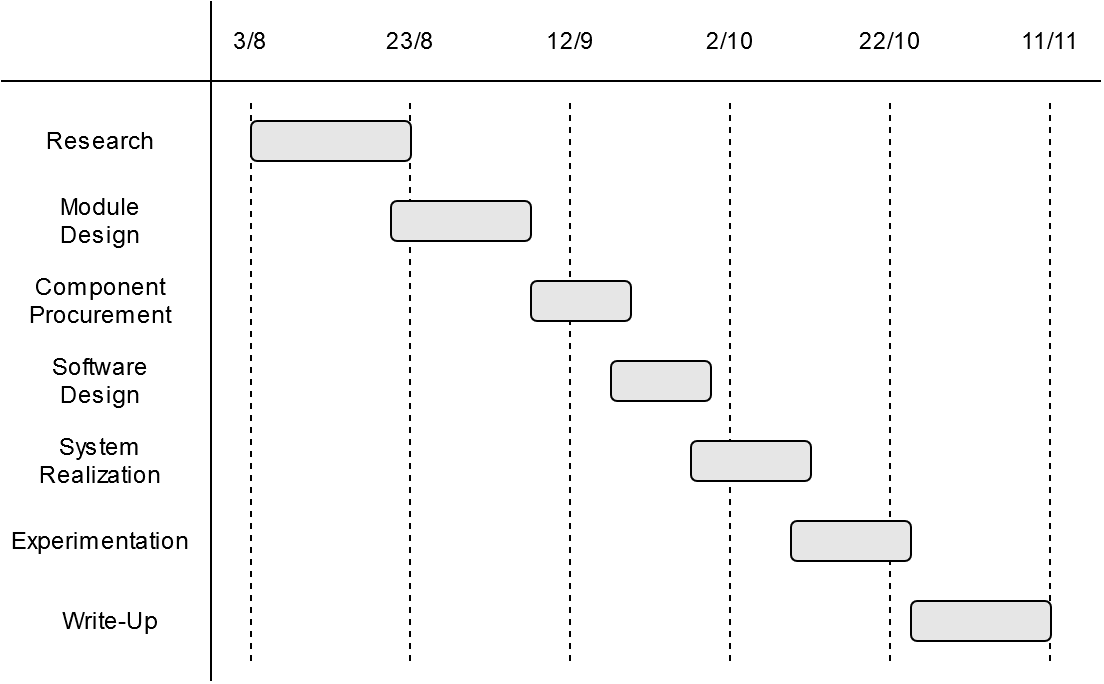
\includegraphics[width=0.8\linewidth]{figures/introduction/gantt_chart.png}
	\caption{Gantt Chart - Time distribution across aspects of the project}
	\label{fig:gantt_chart}
\end{figure}

An initial period will be dedicated to research in the relevant fields of study. Then time will be spent designing the various hardware modules, after which the components will be procured. Software development will begin during the component procurement period. After this period, the modules will be realized. The remaining time will be split between experimentation and the report write-up.